%!TEX program = xelatex
% 完整编译: xelatex -> biber/bibtex -> xelatex -> xelatex
\documentclass[lang=cn,a4paper,chinesefont=founder,bibend=bibtex]{shu-lab-report}
% * 更多配置选项
% \documentclass[lang=cn,a4paper,zihao=-4,chinesefont=founder,bibend=bibtex]{elegantpaper}

% 本文档命令
\usepackage{array}
\newcommand{\ccr}[1]{\makecell{{\color{#1}\rule{1cm}{1cm}}}}
\renewcommand{\lstlistingname}{代码}

\begin{document}

%%%%%%%%%%%%%%%%%%%%%%%%%%%%%
%% The Cover Page
%%%%%%%%%%%%%%%%%%%%%%%%%%%%%

\thispagestyle{empty}

~\\

\vspace{3cm}

\begin{figure}[!htbp]
  \centering
  
\includegraphics[width=10cm]{image/shulogo.png}
\end{figure}

\centerline{\large{\textbf{SHANGHAI  UNIVERSITY}}}

\vspace{8mm}

\centerline{\kaishu\Huge{\textbf{数据库原理(二)实验报告}}}

\vspace{8mm}

\vspace{5cm}

\begin{center}
  \renewcommand\arraystretch{2}
  \begin{tabular}{r c}
    \makebox[8em][s]{\LARGE{学号姓名}} & \LARGE{20121034胡才郁} \\  \cmidrule(l){2-2}
    \makebox[8em][s]{\LARGE{日期}}   & \LARGE{2023年5月21日}  \\ \cmidrule(l){2-2}
  \end{tabular}
\end{center}

\newpage

%%%%%%%%%%%%%%%%%%%%%%%%%%%%%
%% The Content
%%%%%%%%%%%%%%%%%%%%%%%%%%%%%

\section{项目概述}

在校园中生活中,每一位同学都会遇到这样的问题:在食堂点餐时,由于人数众多,导致点餐拥堵,甚至会因此错过课程;又或者是在宿舍中,同学们想要点餐,但是又不想出门,这时候就需要一个点餐软件。我们设计了这款校园点餐App,名字为鼠鼠取餐。鼠鼠(SHU SHU)与上海大学的简称拼音相似,为这款软件添加了一些趣味,我们为这款软件设计了Logo,如\figref{fig:logo}所示。

\begin{figure}[htbp]
  \centering
  
\includegraphics[width=0.3\textwidth]{image/logo.png}
  \caption{鼠鼠取餐软件Logo}
  \label{fig:logo}
\end{figure}

\section{整体设计}

校园点餐App分为客户端和商家端以及后台管理。其中客户端包含的功能模块有:首页和用户登录/注册,餐厅搜索,点餐,查看订单,查看当前用户经常购买的商品。商家端可以登录、注册,进行扫码并核销订单,查看订单,修改商品库存,修改商店的公告、名称等。

其中,用户首页如\figref{fig:1}所示,用户可以在首页进行登录、注册、搜索餐厅、查看订单、查看推荐商品等操作。

\begin{figure}[htbp]
  \centering
  
\includegraphics[width=0.6\textwidth]{image/1.jpg}
  \caption{用户首页}
  \label{fig:1}
\end{figure}

\newpage

本项目整体的类图如\figref{fig:class-graph}所示。类图中直观的展示了本项目的整体结构。用户可以使用手机登陆,每一个用户可以有多个商品评价,点多个商品订单。订单是订单项的超类,一个商品信息使用商品评价,有着多个订单。每一家餐厅又多个店家,每一个店家有多种商品分类,每一种商品分类下又有多个商品信息。

\begin{figure}[htbp]
  \centering
  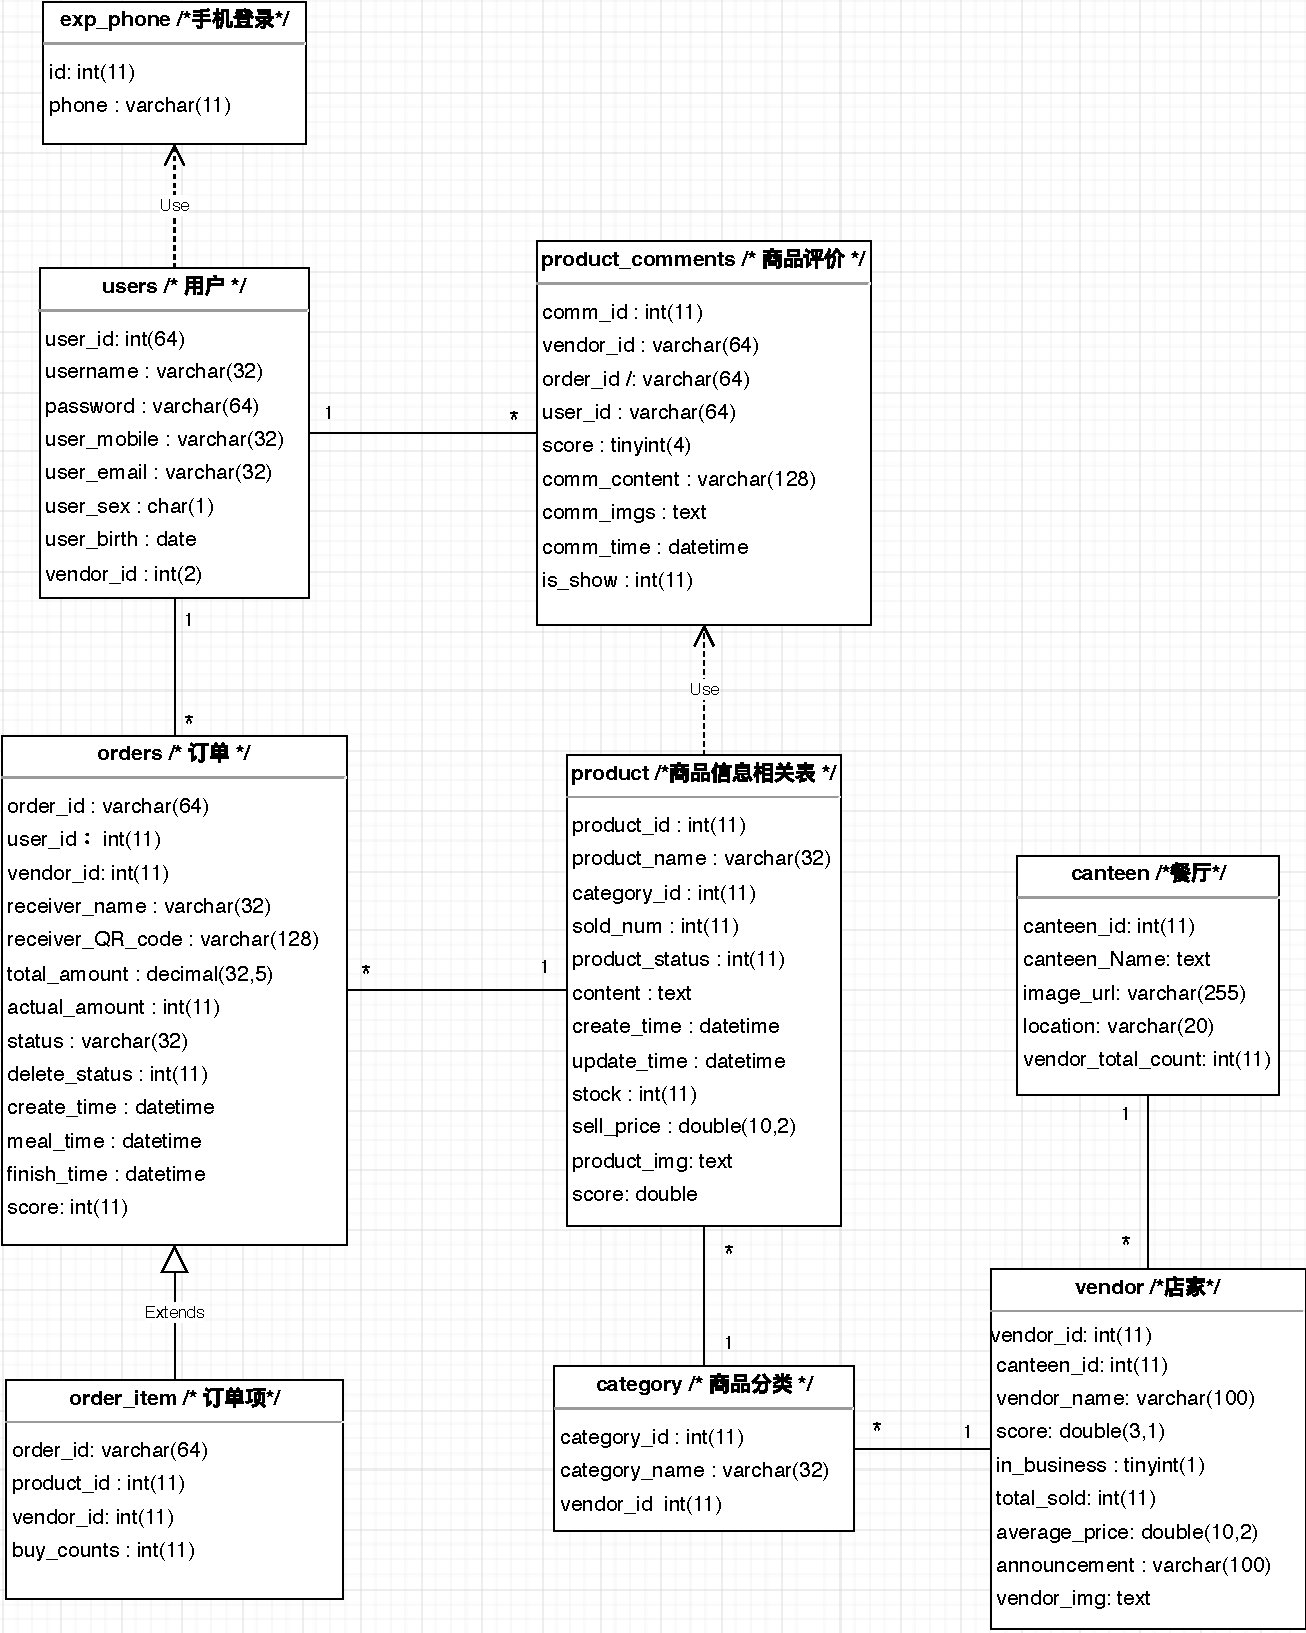
\includegraphics[width=0.8\textwidth]{image/class_graph.pdf}
  \caption{类图}
  \label{fig:class-graph}
\end{figure}

\newpage

本项目整体的ER图如\figref{fig:er-graph}所示。相比较于类图,ER图的优点在于可以直观的展示出实体之间的关系,并且省去了类图中的一些冗余信息。

\begin{figure}[htbp]
  \centering
  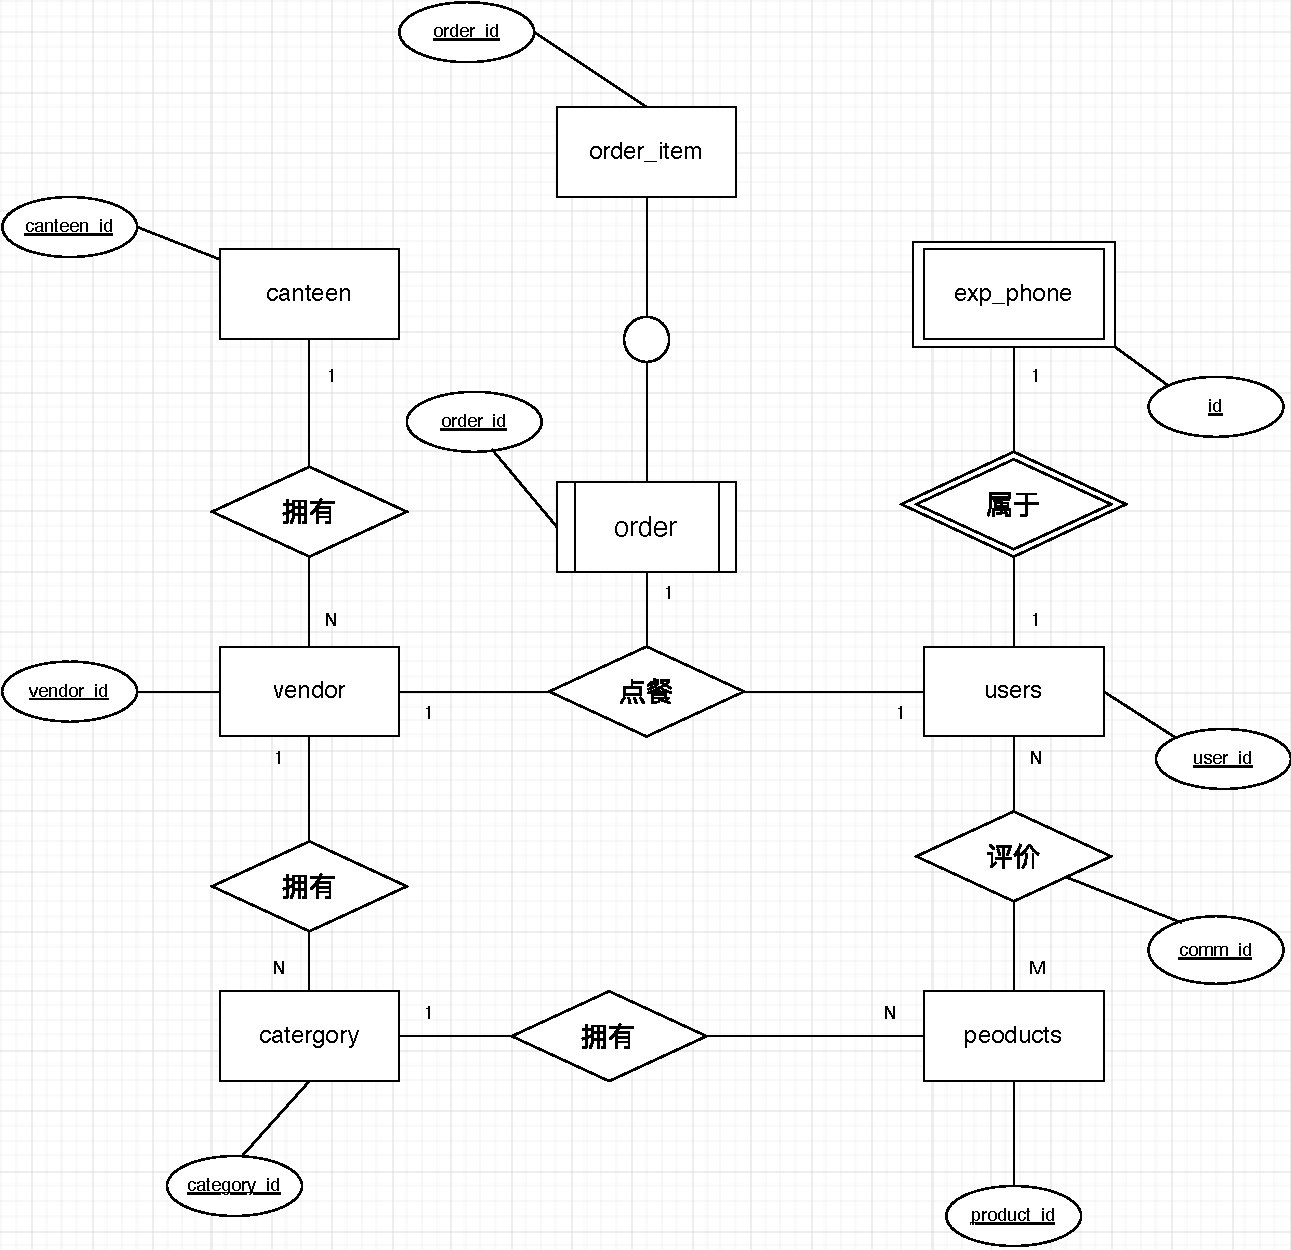
\includegraphics[width=0.8\textwidth]{image/ER.pdf}
  \caption{ER图}
  \label{fig:er-graph}
\end{figure}


将类图、ER图转换为数据库中的表后,共有9张表,如\tabref{tab:my-table}所示。

\begin{longtable}[c]{@{}cc@{}}
  \caption{数据库表设计}
  \label{tab:my-table}            \\
  \toprule
  \textbf{表名}       & \textbf{解释} \\* \midrule
  \endhead
  %
  \bottomrule
  \endfoot
  %
  \endlastfoot
  %
  exp\_phone        & 手机登录        \\
  users             & 用户          \\
  orders            & 订单          \\
  order\_item       & 订单项         \\
  product\_comments & 商品评价        \\
  product           & 商品信息        \\
  category          & 商品分类        \\
  canteen           & 餐厅          \\
  vendor            & 店家          \\* \bottomrule
\end{longtable}

\newpage


\section{功能设计}

\begin{tcolorbox}[colback=orange!5!white,colframe=orange!75!black]
  在本次实验之中,我主要负责了客户端的全部内容,以下提到的功能皆有我参与,接下来按照功能模块进行介绍。
\end{tcolorbox}


\subsection{登录/注册}

登录界面使用了最常见的手机号登录并默认注册的模块设计,当用户输入正确的手机号码并点击发生验证码之后,系统会自动调用发送验证码模块将验证码发送至用户手机上。用户输入验证码之后,点击登录即可跳转到用户界面。

\begin{figure}[htbp]
  \centering
  
\includegraphics[width=0.6\textwidth]{image/2.jpg}
  \caption{登录界面}
  \label{fig:2}
\end{figure}

登录功能的实现原理是:当用户点击发送验证码之后,系统会自动调用发送验证码模块向第三方短信服务平台发送请求,我们在后端使用了云片网络提供的手机短信验证码接口。在云片网注册并实名验证之后,可以申请短信签名模板和apikey。所以在调用接口时只需要传入对应的apikey和模板签名以及需要发送的验证码即可给用户发送短信,达到优化用户体验的效果。

此处的实现不仅仅与APP开发技术关系密切,与数据库课程的联系十分紧密。原因是发送之后的验证码会存储在上个学期所提到的Redis数据库中,并且为了保证时效性,每隔一段时间就会自动删除。所以在用户输入验证码之后,我们需要调用Redis数据库的接口,从而获取到用户输入的验证码,然后与发送的验证码进行比对,如果一致,则登录成功,否则登录失败。这利用了Redis这类非关系型数据库相比较于关系型数据库的优势,即速度快,适合存储一些时效性较短的数据。

\newpage

\subsection{首页信息}

首页部分提供了搜索框,店铺介绍等点餐必备的信息。可以看到,首页的设计十分简洁。对于每一个店家,用户打分和价格销量,会显示在店铺封面的介绍中。其中,打分和价格销量是根据用户点评和下单评价、销量统计计算得到的,并非是随机生成的数据。具体的实现部分在之后的触发器中会提到。

\begin{figure}[htbp]
  \centering
  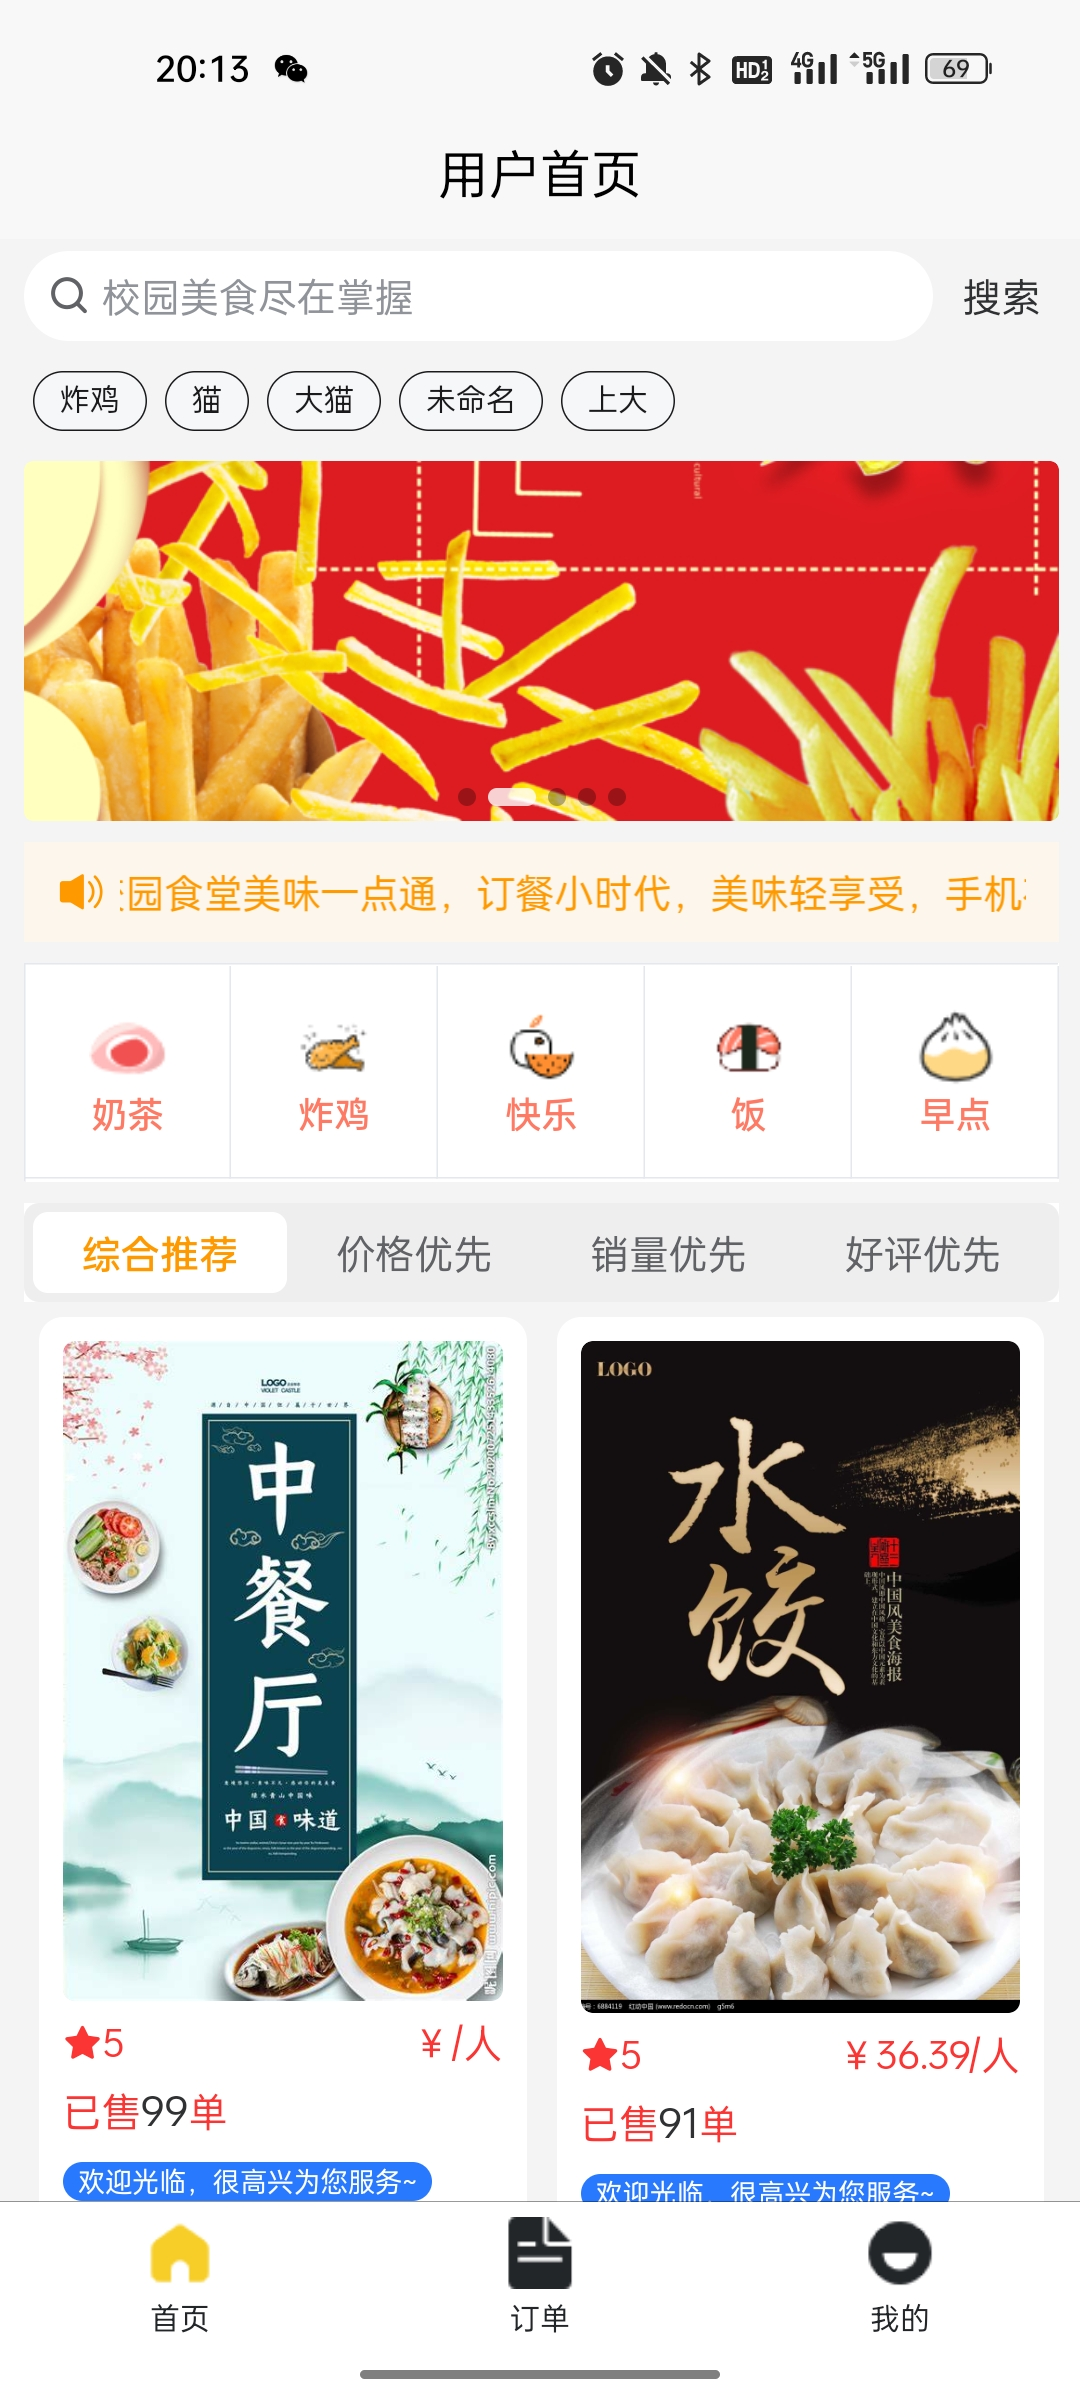
\includegraphics[width=0.4\textwidth]{image/4.jpg}
  \caption{用户首页}
  \label{fig:4}
\end{figure}

并且,为了尽量逼真上海大学内的真实情况,我们的全部数据来源为真实数据,例如对于食堂信息,我们真实的获取了上海大学内益新、尔美、山明、水秀等食堂的店铺信息。例如在\figref{fig:4}中所展示出来的店铺“中餐厅”就是上海大学益新食堂内的一家店铺。其余更多信息,可以根据\figref{fig:5}中的数据证明,“快乐食间”系列为尔美食堂内的店铺。

\begin{figure}[htbp]
  \centering
  
\includegraphics[width=0.4\textwidth]{image/5.jpg}
  \caption{部分真实的商家信息}
  \label{fig:5}
\end{figure}

\newpage

\subsection{美食搜索}

在商家搜索页面可以搜索想吃的美食,并且对于各个商家提供了综合排序、销量优先、评分优先的筛选方式,并且会记录用户的历史美食搜索信息,方便用户二次查找。

\begin{figure}[htbp]
  \centering
  
\includegraphics[width=0.55\textwidth]{image/3.jpg}
  \caption{搜索功能}
  \label{fig:3}
\end{figure}

并且为了保证时效性,每次搜索过的关键词,都会自动记录在这个用户的历史搜索记录中,方便用户二次查找。

\newpage

\subsection{点餐功能}

进入某一个店家后,可以点餐操作,由于只是实验,并没有做真实的支付功能。在这个订单中可以选择领餐时间、姓名、手机号等等,并可以在订单的备注中注明口味等其余要求。当确认支付后,系统根据此订单的价格,点餐成功后该商店人均价格与销售量会实时改变。并且人均价格这个指标也可以作为查询商家时的筛选标准。

\begin{figure}[htbp]
  \centering
  
\includegraphics[width=0.55\textwidth]{image/6.jpg}
  \caption{店铺内容与订单界面}
\end{figure}

在确定订单部分可以选择具体的领餐时间、领餐地点,填写手机号、姓名等,并且可以添加备注。

当支付成功之后,将返回用户取餐吗,客户使用二维码即可在商家端部分进行核销。下图左为核销之前的代取餐状态,图右为已核销,订单完成状态。

\begin{figure}[htbp]
  \centering
  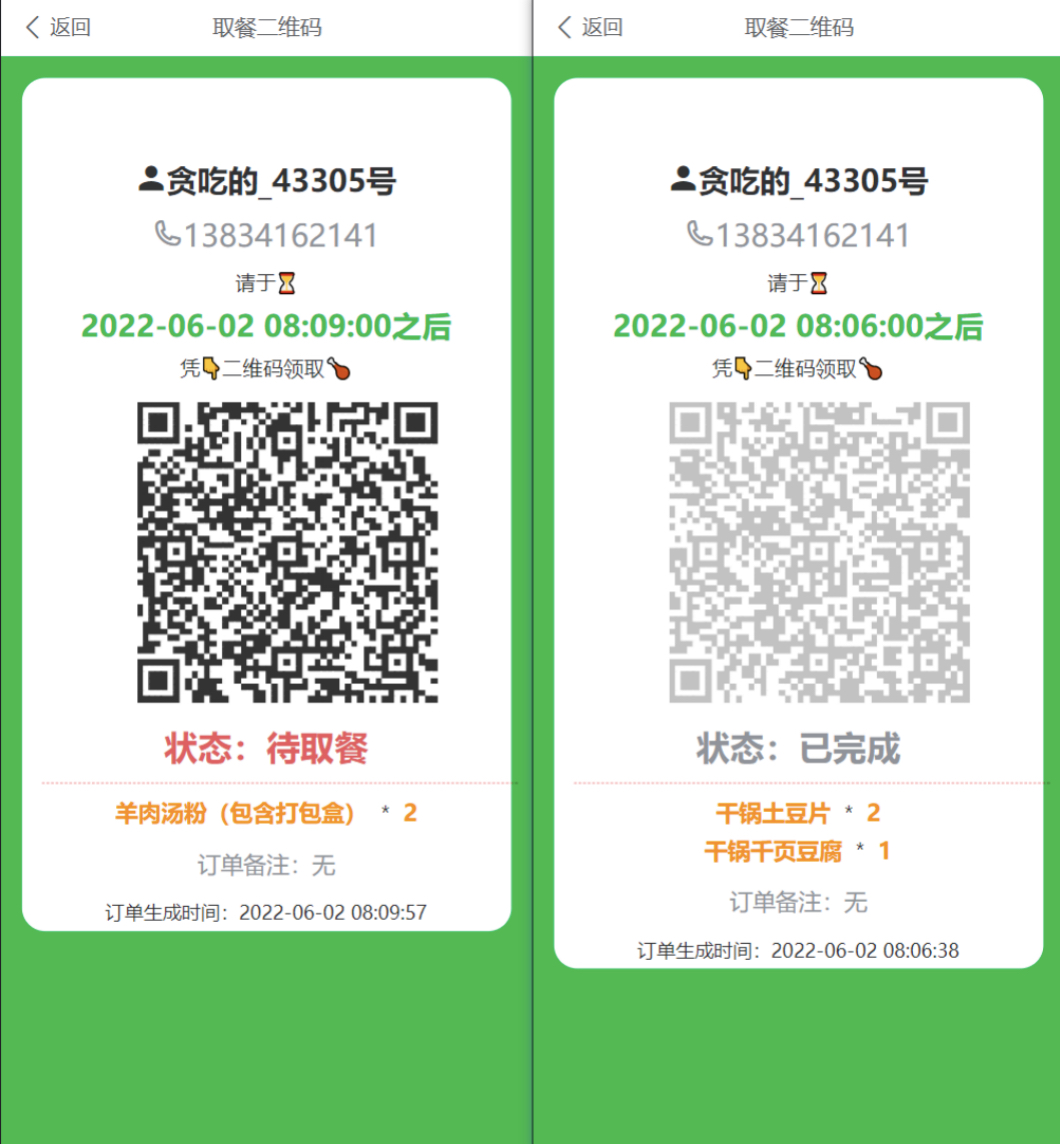
\includegraphics[width=0.4\textwidth]{image/7.jpg}
  \caption{取餐码核销界面}
\end{figure}

而在订单完成后,系统自动会将记录添加到最近常买模块中,这样用户就可以快捷跳转到他常买的商家,方便用户的使用。

\begin{figure}[htbp]
  \centering
  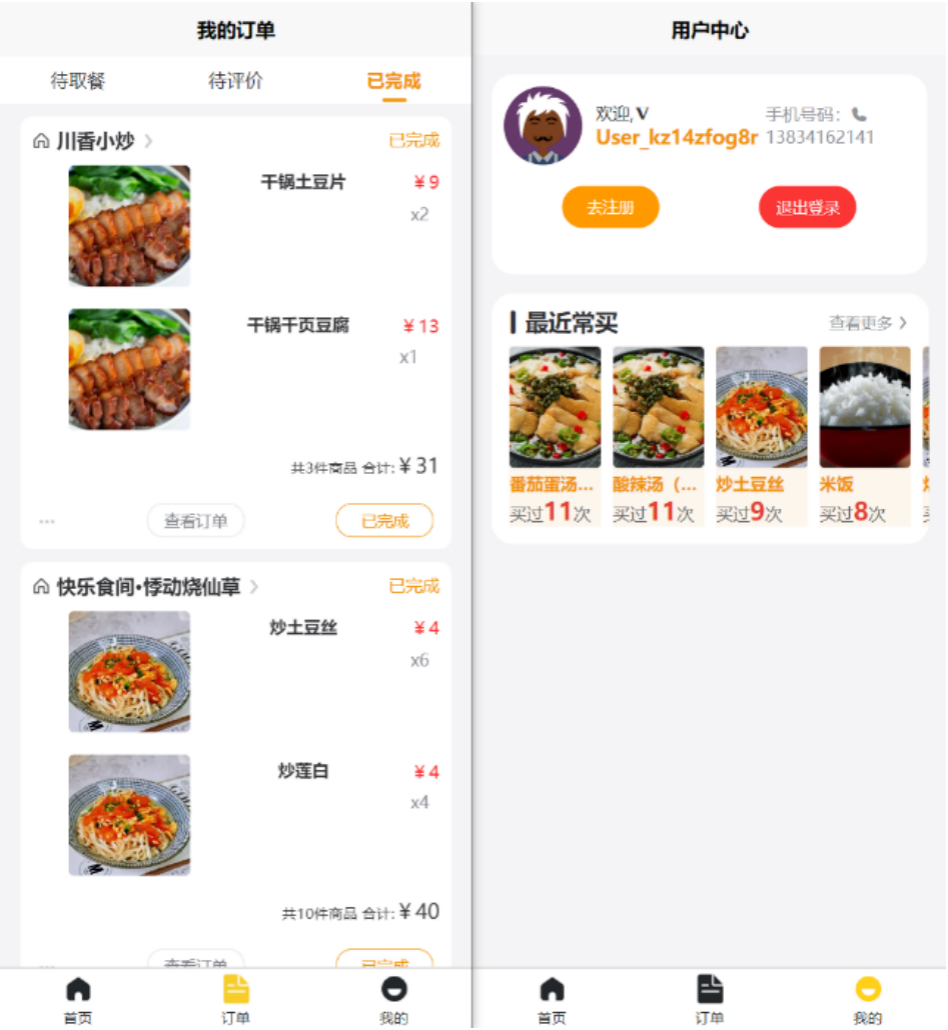
\includegraphics[width=0.5\textwidth]{image/8.jpg}
  \caption{最近常买模块}
\end{figure}

\subsection{订单评价功能}

在订单的评论界面,对于购买过商家进行打分与评论,并且可以上传多张图片。此分数会实时影响该店家的得分,并且作为查找时的筛选依据。并且,对于每一个订单,用户只能评论一次,防止刷分,在用户完成评价后,此订单会自动转变为已完成状态。

\begin{figure}[htbp]
  \centering
  
\includegraphics[width=0.45\textwidth]{image/9.jpg}
  \caption{订单评价界面}
\end{figure}

\section{技术介绍}

\begin{tcolorbox}[colback=orange!5!white,colframe=orange!75!black]
  在本次实验之中,我主要负责完成权限管理、触发器部分和后端开发任务。
\end{tcolorbox}

\subsection{触发器}

触发器是数据库中的一种特殊对象,它是由事件驱动的特殊存储过程。当满足某个事件时,触发器会自动执行。触发器可以用来保证数据的完整性,也可以用来实现业务逻辑。此处介绍在开发过程中我使用到的两个触发器。

\subsubsection{触发器1}
\begin{lstlisting}[language=SQL]
# 元组级触发器
create definer = root@`%` trigger block_insert
    before insert
    on canteen
    for each row
BEGIN
  DECLARE msg VARCHAR(255) DEFAULT 'New data cannot be added to the canteen table.';
  SIGNAL SQLSTATE '45000' SET MESSAGE_TEXT = msg;
END;
\end{lstlisting}

此处的触发器是针对于食堂表的,针对于目前学校情况,假设学校不会增加食堂,因此设置触发器,当有插入操作时,触发器会报错,阻止插入操作,保证了数据的完整性。

\subsubsection{触发器2}

\begin{lstlisting}[language=SQL]
create definer = root@`%` trigger update_vendor
  after update
  on orders
  for each row
BEGIN
  IF NEW.vendor_id IS NOT NULL THEN
      UPDATE vendor SET total_sold = total_sold + 1, average_price = ((average_price * total_sold) + NEW.actual_amount) / (total_sold + 1)
      WHERE vendor_id = NEW.vendor_id;
  END IF;
END;
\end{lstlisting}

此处的触发器是针对于订单表的。由于商家表中的销售量与人均价格是根据订单表中的数据计算得到的,并且此两个数据是经常被查询的,因此在订单表中设置触发器,当订单表中的某一条记录被更新时,触发器会自动执行,更新商家表中的销售量与人均价格,保证了数据的一致性。这也印证了在首页展示时,商家的销售量与人均价格是实时更新的。

\subsection{权限管理}

MySql中的权限管理可以使得不同的用户拥有不同的权限,从而保证了数据库的安全性。在本次实验中,我设置了三个用户,分别是admin、merchant、customer。例如,管理员 ‘admin’ 拥有数据库 ‘cloud\_order’ 的所有权限;商家 ‘merchant’ 可以进行商品表 ‘products’ 的 SELECT、INSERT、UPDATE、DELETE 操作;用户 ‘user’ 仅可以进行商品表 ‘products’ 的 SELECT 操作。

\begin{lstlisting}[language=SQL]
CREATE USER admin WITH PASSWORD 'admin_password';
CREATE USER merchant WITH PASSWORD 'merchant_password';
CREATE USER user WITH PASSWORD 'user_password';

CREATE ROLE admin_role;
CREATE ROLE merchant_role;
CREATE ROLE user_role;

GRANT admin_role TO admin;
GRANT merchant_role TO merchant;
GRANT user_role TO user;

GRANT admin_role, merchant_role TO merchant;

-- 管理员拥有所有权限
GRANT ALL PRIVILEGES ON DATABASE myapp TO admin;

-- 商家端可以修改、删除、增加商品表
GRANT SELECT, INSERT, UPDATE, DELETE ON products TO merchant;

-- 用户端可以浏览商品表
GRANT SELECT ON products TO user;
\end{lstlisting}


\subsection{后端开发技术栈}

后端开发工具IDEA,数据库采用Mysql,数据库连接池采用Druid。Dao层使用Mybatis-Plus,Mybatis-Plus(简称 MP)是一个 Mybatis 的增强工具,在 MyBatis 的基础上只做增强不做改变,为简化开发、提高效率而生。工具类采用了Hutools,包含了常用的uuid生成,json数据转换等。缓存采用Redis,Redis是一个开源的使用ANSI C语言编写、支持网络、可基于内存亦可持久化的日志型、Key-Value数据库,并提供多种语言的API。服务器采用Nginx,Nginx是一个高性能的HTTP和反向代理服务器,也是一个IMAP/POP3/SMTP服务器。本次的所有数据都放到了华为云服务器上,也因此我们开发的APP可以在任何地方使用。

% Please add the following required packages to your document preamble:
% \usepackage{longtable}
% Note: It may be necessary to compile the document several times to get a multi-page table to line up properly
\begin{longtable}[c]{|c|c|}
  \caption{后端开发技术栈}
  \label{tab:1}                    \\
  \hline
  SpringBoot      & Spring容器+MVC框架 \\ \hline
  \endhead
  %
  MyBatis         & ORM框架          \\ \hline
  MyBatisPlus     & 数据层代码生成        \\ \hline
  Nginx           & 静态资源服务器        \\ \hline
  Druid           & 数据库连接池         \\ \hline
  Lombok          & 简化对象封装工具       \\ \hline
  Redis           & 缓存             \\ \hline
  Hutools         & 工具类            \\ \hline
  Mysql-connector & Mysql连接池       \\ \hline
\end{longtable}

\section{感受与体会}

随着这个项目的开发结束,也宣告着这学期的结束,我也马上要结束大学的第三个学年。《数据库原理》作为计算机专业的基本功,值得我们重视学习。作为一名计算机专业的学生,我们不仅需要掌握基本的理论知识,更需要通过实践来提高自己的实践能力和技术水平。通过这个项目,我学会了如何将理论应用到实践中,理解了软件开发的流程和方法。

然而,在开发这个看似简单的APP的过程中,实际上也遇到了许多的问题。例如,在一开始时,数据库迟迟无法上云,导致刚开始的开发进度大大的拖慢了。我们本次开发为了保证进度的统一,也使用了目前主流的版本控制工具git帮助我们进行协作,但是在合并代码的过程中也遇到了一些冲突的问题。

通过这次实践,我深切地感受到了数据库的重要性和版本控制工具的便利性。同时,也学会了如何提高团队协作的效率和解决问题的能力。除此之外,我还学习了一些APP开发和UI设计的基本技能,这些技能对我未来的职业发展也是非常有帮助的。

回顾这学期的学习生活,我认为最大的收获不仅仅是知识的积累,更重要的是培养了我的自信心,当看到自己开发的软件运行起来,当为自己开发的软件设计Logo,这样的时刻是十分自豪的。

\end{document}
